% !TeX program = lualatex
\documentclass[DIV=12, parskip=half, fontsize=12pt, a4paper]{scrartcl}

%\usepackage[utf8]{inputenc}
%\usepackage[T1]{fontenc}    % Font-Encoding
%\usepackage{lmodern}        % LModern font
\usepackage[ngerman]{babel} % deutsche Lokalisierung
%\usepackage{graphicx}       % Einbindung von Bildern
\usepackage{pdfpages}

\usepackage{lineno}         % Nummerierung der Zeilen
\usepackage{csquotes}       % bessere Anführungszeichen
%\usepackage{eurosym}        % Euro-Zeichen setzen
%\usepackage[normalem]{ulem} % Durchstreichen von Text-Passagen
\usepackage[shortlabels]{enumitem} % bessere Aufzählungen mit Kurzschreibweise der Labels

\usepackage{pdfpages}       % erlaubt das Einbinden von Seiten anderer PDF-Dateien

\usepackage{draftwatermark}
\SetWatermarkText{Entwurf}



\title{Änderungsantrag zum Antrag zur Neufassung der Fachschaftswahlordnung (FSWO)}
\author{Fachschaftenkonferenz}
\date{18.\ Januar 2021}

\begin{document}
  \maketitle
  Das SP möge auf Vorschlag der Fachschaftenkonferenz beschließen:

  \begin{linenumbers}
    Im \enquote{Antrag zur Neufassung der Fachschaftswahlordnung (FSWO)} vom 9.\ November 2020 wird die beigefügte Wahlordnung  wie folgt geändert:

    \begin{enumerate}[1.]
    	\item \S 11 Absatz 6 wird wie folgt neu gefasst:
    		\begin{enumerate}[(1)] \ttfamily
    		\setcounter{enumii}{5}
    		\item Die Wahlleitung soll die ihr obliegenden Aufgaben selbst wahrnehmen.
    			In Einzelfällen kann sie einzelne ihrer Aufgaben nach Absprache auch anderen Wahlausschussmitgliedern übertragen.
    		Über diesen Vorgang ist Protokoll zu führen.
    		\end{enumerate}
    	\item \S 28 Absatz 10 wird wie folgt neu gefasst:
    		\begin{enumerate}[(1)] \ttfamily
	    		\setcounter{enumii}{9}
	    		\item Eine Festlegung nach Absatz 1, die nach Bestellung des Wahlausschusses hinzugefügt oder gestrichen wird,
	    			entfaltet keine Wirkung mehr für diese Wahl.
	    	\end{enumerate}
    \end{enumerate}
  \end{linenumbers}

\vspace{1em}
\textbf{Begründung:}\par
Beide Punkte sind Empfehlungen der SP-SGO-Ausschusses, denen sich die FK gerne angeschlossen hat.
Der zweite Punkt ist nur redaktionell.

  \vspace{1em}
  \textit{Ausgefertigt aufgrund des Beschlusses der Fachschaftenkonferenz vom 18.\ Januar 2021.}

  Bonn, den 18.\ Januar 2021 \\
  Philipp Wippermann \\
  {\scriptsize Vorsitzender des Fachschaftenkollektivs, Fachschaftenreferent}

%  \clearpage
%  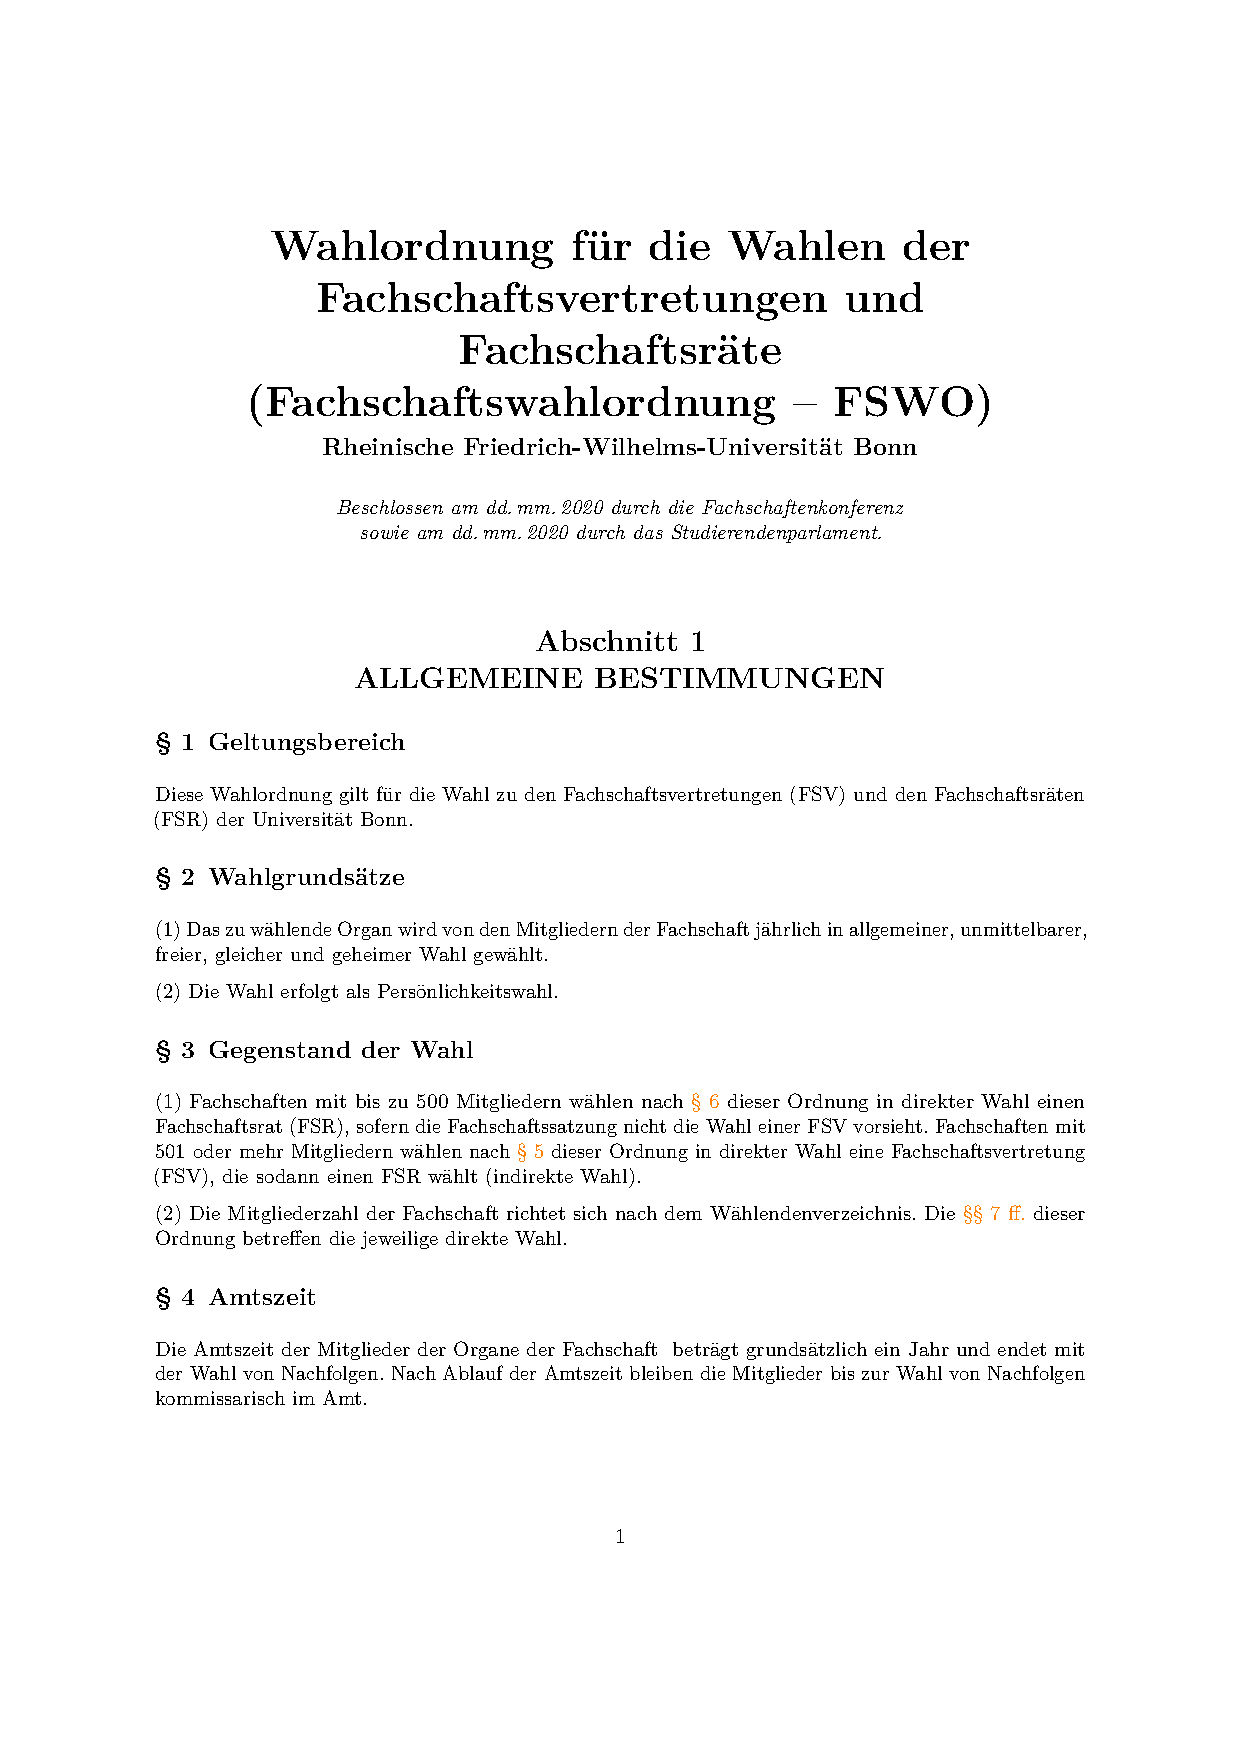
\includepdf[pages=-]{FSWO-Entwurf-ohne-Anmerkungen}
\end{document}
